%===============================================================================
%===============================================================================
%
\subsection{Example-0101}
%
%===============================================================================
%
\subsubsection{Model}
%
We solve the following equation,
%
\begin{align}
    \ldots & &&\Omega \in [ldots] \times [\ldots],
\end{align}
%
with boundary conditions
%
\begin{align}
    \ldots & && \ldots, \\
    \ldots & && \ldots.
\end{align}
%
2D: specify thickness, Young's modulus and Poisson's ratio.
%
%===============================================================================
%
\subsubsection{Results}
%
\begin{figure}[h!]
    \centering 
    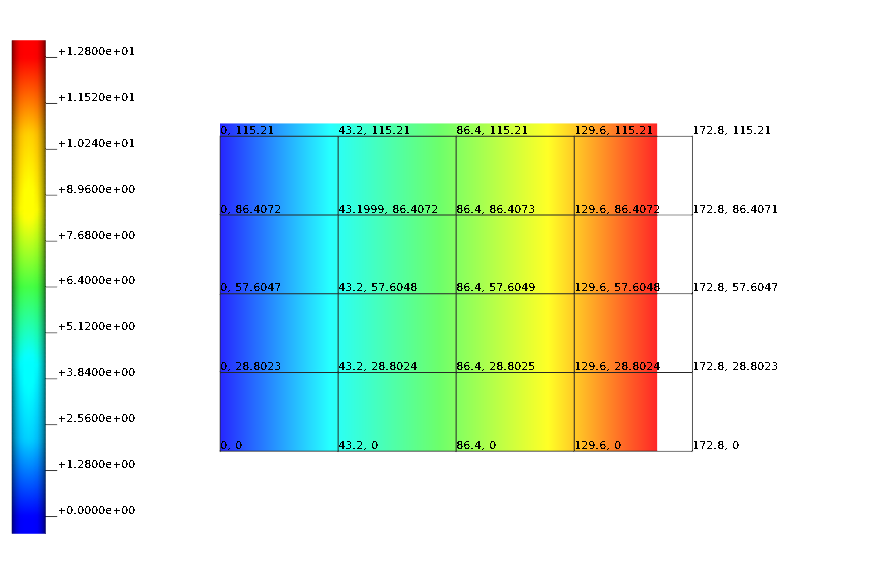
\includegraphics[width=\columnwidth]{examples/example-0101/figures/example.png} 
    \caption{Results.}
    \label{example-0101-fig}
\end{figure}
%
%===============================================================================
%===============================================================================
